\documentclass[11pt]{article}

\usepackage{geometry}
\geometry{letterpaper}

\usepackage{graphicx}
\usepackage{amssymb}
\usepackage{epstopdf}
\usepackage{caption}
\usepackage{subcaption}
%\usepackage{natbib}
\usepackage{amssymb, amsmath}
\usepackage{mcode}

\DeclareGraphicsRule{.tif}{png}{.png}{`convert #1 `dirname #1`/`basename #1 .tif`.png}
%\title{SIG - Sequential Investment Game}
%\author{Simon Zimmermann, Fabian Keller, Sebastian Klotz}
%\date{date}
\begin{document}
\thispagestyle{empty}
\begin{center}

\includegraphics[scale=1]{ETHlogog.png}\\
\bigskip
\bigskip
\bigskip
\LARGE{ Lecture with Computer Exercises:\\ }
\LARGE{ Modelling and Simulating Social Systems with MATLAB\\}
\bigskip
\bigskip
\small{Project Report}\\
\bigskip
\bigskip
\bigskip
\bigskip
\begin{tabular}{|c|}
\hline
\\
\textbf{\LARGE{SIG - Sequential Investment Game}}\\
\\
\hline
\end{tabular}

\bigskip
\bigskip
\bigskip
\LARGE{Fabian Keller, Sebastian Klotz \& Simon Zimmermann}\\
\bigskip
\bigskip
\bigskip
\bigskip
\bigskip
\bigskip
\bigskip
\bigskip
Zurich, December 2014\\
\end{center}

%%%%%%%%%%%%%%%%%%%%%%%%%%%%%%%%%%%%%%%%%%%%%%%%%
\begin{center}
	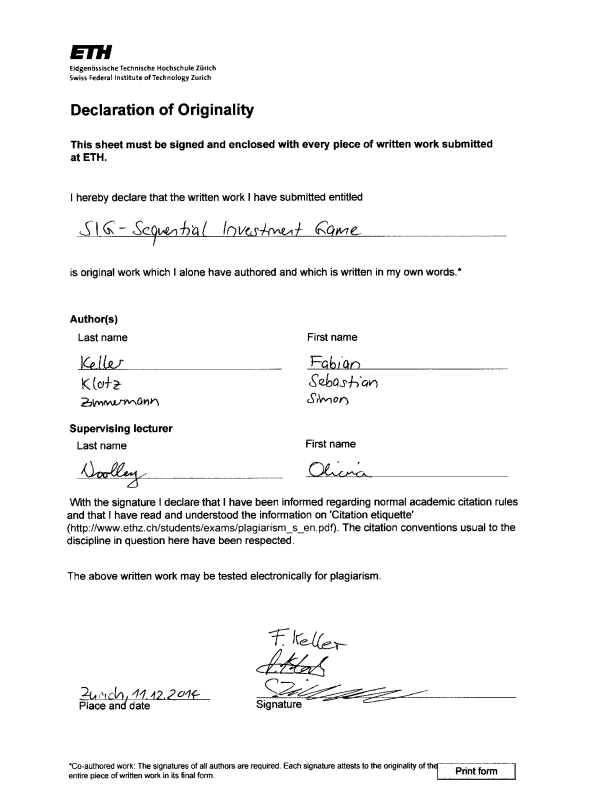
\includegraphics[scale=0.95]{Declaration_of_originality_signed_final}
\end{center}

\newpage

\section*{Agreement for free-download}
\bigskip
\bigskip
\large We hereby agree to make our source code for this project freely available for download from the web pages of the SOMS chair. Furthermore, we assure that all source code is written by ourselves and is not violating any copyright restrictions.

%\begin{center}
%\bigskip
%\bigskip
%\begin{tabular}{@{}p{3.3cm}@{}p{6cm}@{}@{}p{6cm}@{}@{}p{6cm}@{}}
%\begin{minipage}{3cm}
%\end{minipage}
%&
%\begin{minipage}{6cm}
%\vspace{2mm}\large Simon Zimmermann
%\vspace{\baselineskip}
%\end{minipage}
%&
%\begin{minipage}{6cm}
%\large Fabian Keller
%\end{minipage}
%&
%\begin{minipage}{6cm}
%\large Sebastian Klotz
%\end{minipage}
%\end{tabular}
%\end{center}

\begin{center}
\bigskip
\bigskip
\setlength{\tabcolsep}{15pt}
	\begin{tabular}{l c r}	
		Fabian Keller  &  Sebastian Klotz  &  Simon Zimmermann
	\end{tabular}
\end{center}
\newpage

%%%%%%%%%%%%%%%%%%%%%%%%%%%%%%%%%%%%%%%
% IMPORTANT
% you MUST include the ETH declaration of originality here; it is available for download on the course website or at http://www.ethz.ch/faculty/exams/plagiarism/index_EN; it can be printed as pdf and should be filled out in handwriting
%%%%%%%%%% Table of content %%%%%%%%%%%%%%%%%

\tableofcontents
\newpage

%%%%%%%%%%%%%%%%%%%%%%%%%%%%%%%%%%%%%%%

\section{Abstract}
As part of the GESS-course "Modelling and Simulating Social Systems with MATLAB" at ETH Zurich this project tries to find an optimal strategy for the sequential investment game for two players. To find such a strategy different models of the problem have been implemented and simulated in MATLAB. The basic result of the project is that it seems that no better strategy than the Kelly-criterion ceases to exist. 

\section{Individual contributions}
Every member of the group for this exercise contributed about the same amount of work and effort in every phase of the project. We all met and stuck our heads together to create new ideas and to take a critical point of view on another members ideas. \\
However every team member had his own field of responsability. Fabian was working with the code a lot, Simon did a big part of administrative work and Sebastian did the basic layout of the report.

\section{Introduction and Motivations}
We took the GESS course "Modelling and Simulating Social Systems with MATLAB" for several reasons. All team members are studying Mechanical Engineering. That's the reason why we have to use the software MATLAB a lot. So we decided to take that course to improve our MATLAB knowledge and skills. Furthermore none of us has written any report using LATEX. In regard to the upcoming bachelor and master thesis, we thought that it would be a good idea to gather some experiences in this tool as well. Because our studies are mainly based on technical approaches we were interested in doing some social research to get some knowledge in this area. \\
For our project work we took the topic "Game theory". We all have heard about it before but neither had much background nor had worked in this field before, but we were interested in learning more about the content and the possible applications of this theory. So we decided to take the challenge of doing some self-studies based on our research question.

\section{Theoretical Background}
\subsection{Game Theory}
The base for the following content is game theory. Thinking about our every day lives, decisions are made all the time. Especially if it comes to decisions concerning investments one better thinks twice. Now if we knew all the things other people are about to do we could adjust our decisions so we get the best results for us in every occasion. In reality, as we all know, people are irrational. Driven by our feelings and the fact that we don't know everything about each other is the cause for our irrationality, which makes us human. This is one of the key elements in game theory. It's goal is to model conflicts between rational parties.  It is about interactions between players. \\
One of the key elements is the so called Nash-Equilibrium which is a point where one player has no intention to change his strategy because he has no (additional) benefit if he did so. \\
Game theory plays a big role in modelling problems in economics, computer science, biology and many more. There are many branches that game theory can be divided into but the one we're looking into more deeply is a kind of evolutionary game theory. \\
Evolutionary game theory originates in the idea of modelling biological circumstances. It differs from the common game theory by the fact that players are not aiming for the maximum income but rather try to find the optimum strategy to beat the opposing player. Players are looking through the strategies played in previous games and try to optimize them. It doesn't really matter how much of a currency one player wins as long as he wins against his opponent.
 
\subsection{Kelly criterion}
John Larry Kelly, Jr. (1923-1965),when working for the Bell Labs, found an algorithm which would maximize the winnings for one player, that is playing against a ''bank'' (and not against another player). Given a certain probability of winning $p$ he derived the formula
$$f=\frac{p(b+1)-1}{b}$$
where $b$ is the amount of currency you get back in addition to the wagered amount $f$. In the case that you get back the entire amount you wagered $(b=1)$ the formula reduces to the simple form
$$f=2p-1$$
If for example the probability of winning a game is $p=0.6=60\%$ the amount of currency wagered would be $f=2\cdot0.6-1=0.2=20\%$. That is, one should wager $20\%$ of his holdings to get the maximum in the long run.

\subsection{Sequential Investment Game}
The Kelly criterion is a good start if there's only one player. With the Sequential Investment Game (SIG) there come some additional conditions and more players. To keep the problem simple there'll be just one more player but the problem could be for any number of $n$-players. In addition the probability of winning $p$ will be constant throughout the entire game as well as the amount of currency both players are starting with $k=100$. The whole game consists of $r=1000$ rounds and each round of $t=10$ turns. Each player chooses a strategy and plays $10$ turns during which their strategy doesn't change. After those $10$ turns the holdings of both players are compared and the one who's holding more currency wins the round. After one round they can both change their strategy if they want to. Before each round the holdings of each player are set back to $k=100$. The only point where the players get to know something about the other ones playstyle is after each round. A player only sees that he wins or loses and the difference in currecy between him and the other player. This goes on until all $1000$ rounds are played and the game ends. The player who has won more rounds wins the whole game.

\subsection{Ficticious Play}
Ficticious play (FP) belongs to the branch of evolutionary game theorie. The basic idea of FP is that players are not acting completely rational. The players' goal is to win the game no matter how much currency they actually win. Their strategies depend on the other players history of strategies played. Each player tries to beat the other players strategy. FP is one approach to choose the right strategy for the players playing the SIG. Some inspirationes were taken from the rules of FP.
\pagebreak
\section{Research question}
We want to expend the problem of the Kelly criterion - which is just for one player - to a problem where two players are playing the game against each other. Unlike the Kelly criterion there is no closed form solution anymore. So we try to solve this problem with simulations. Our research question is:''Is there a Nash equilibrium for our expended problem?'' meaning that we try to figure out if there is a strategy where one or both players (we don't know yet) have no intention of changing the strategy while playing the game for several times. If there is a strategy we want to specify how this strategy looks like and find some reasons why it looks like this. For this complex problem we have to fix some play rules and make  assumptions for simplification which are all explained below.

\section{Implementation}
The whole project was a continuous working process. We developed an idea, worked on it, got further experiences and tried to implement new ideas based on this. So we got - besides some fine tuning - four major attempts.
The implementation of the core game remained the same in every version but the way the players chose their strategies changed.\\
\textbf{Remark:}\\
In the following subsections there's being talked a lot of ''strategies''. So what is a strategy and how does it look like? A strategy is, if not mentioned differently, kept over one round. So a player chooses one strategy and plays it through. For an example of a strategy see Fig. \ref{strategy example} .
\begin{figure}[h]
	\centering
	\begin{tabular}{|c|c|c|c|c|c|c|c|c|c|}
	\hline
	turn $t$ & 1 & 2 & 4 & 5 & 6 & 7 & 8 & 9 & 10\\
	\hline
	bet [\%] & 20 & 40 & 30 & 60 & 34 & 56 & 23 & 90 & 2\\
	\hline
	\end{tabular}
	\caption{Example for a strategy}
	\label{strategy example}
\end{figure} 

\subsection{Version 1: Reference Matrix}
This version is the very basic and first attempt in which we tried to solve at least some part of the problem.

\subsubsection{Assumptions \& Implementation}
We implemented the basic structure of the game: The players start with a strategy close to Kelly (for starters we start with Kelly because at this point we just know that this strategy makes sense). Each player sticks to his chosen strategy for one round. The winner gets a new strategy which randomly shifts a little bit. The loser mimes his opponents strategy. We use here one first approach of fictitious play, namely that one player assumes that the other player will play the same strategy as he did before because he has been successful.

As there was no such thing like learning from previous games we asked ourself how we could ''teach'' the players what strategy they should use. So we decided to give them a kind of reference table (see Fig. \ref{refernce table}). This table contains all the possible strategy combinations for both players. The idea is that both players were granted access to this table and could look up which strategy they should pick to beat the opponent. So this reference table could be seen as a kind of "experience" we try to give the players.

The table is created by simulating games where one bet plays against another bet (for example 1\% against 50\%) for 10000 times. Each time a bet on the x-axis wins it gets a ''point'' and each time it loses one ''point'' is substracted. This way we count the amount of wins of a bet. The players search the table for the opponents bet and choose the bet which has won the most according to the table. He then plays with this bet.
\begin{figure}
	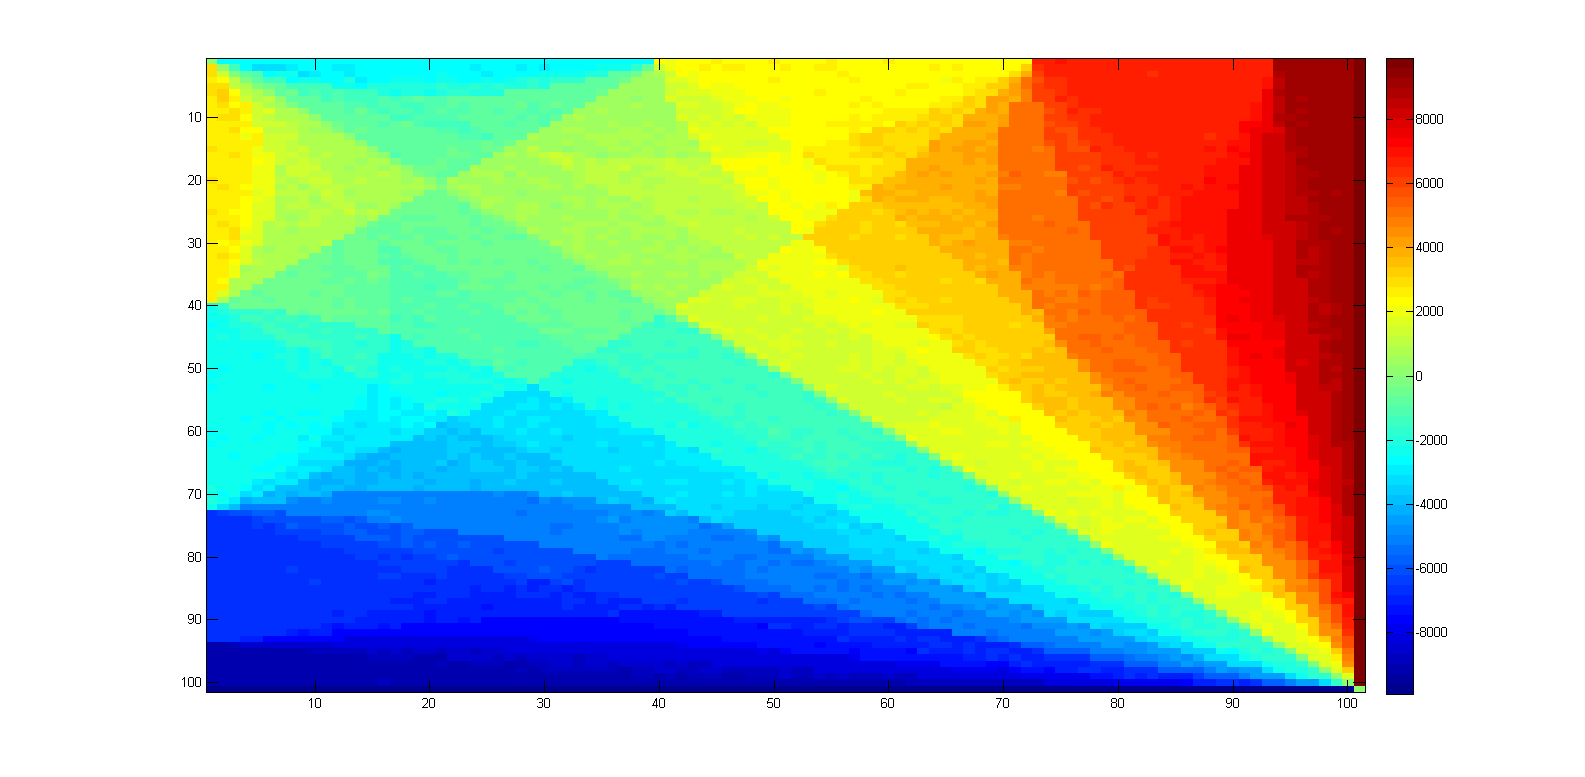
\includegraphics[scale=0.2]{plot_ref_10000_V1.png}
	\centering
	\caption{Reference table}
	\label{refernce table}
\end{figure}

\subsubsection{Results \& Discussion}
The results we get out of the play are not very useful. The whole game seems to be to random to make significant statements. Almost every game was very close to a draw. As we can see in Fig. \ref{Results 1} the scores of the players are, besides some really lucky games, very close to each other. Up to that point we haven't implemented a good strategy counter to compare and judge the strategies.
The evaluation of the reference table leads us to the conclusion that in this way of playing, Kelly is still the best strategy.
\begin{figure}[h]
		\centering
		\begin{subfigure}[b]{0.4\textwidth}
                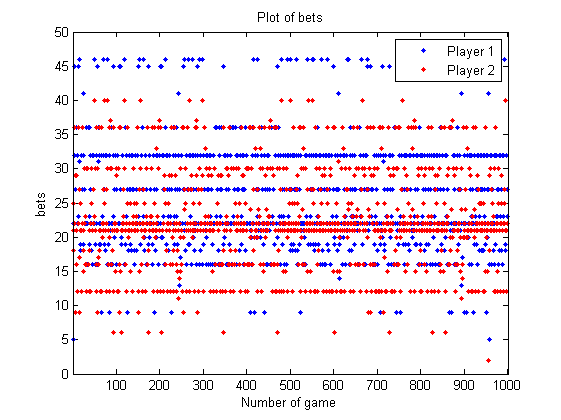
\includegraphics[width=\textwidth]{plot_of_bets_V1}
                \caption{Plot of bets}
                \label{bets 1}
        \end{subfigure}
        \begin{subfigure}[b]{0.4\textwidth}
                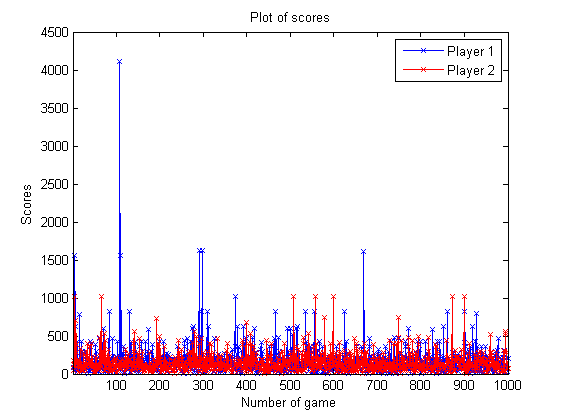
\includegraphics[width=\textwidth]{plot_of_scores_V1}
                \caption{Plot of scores}
                \label{scores 1}
        \end{subfigure}
        \caption{Results of version 1}
        \label{Results 1}
\end{figure}

\subsection{Version 2: Random strategies}
\subsubsection{Assumptions \& Implementation}
With the second version we try to react to the feedback that we got from Olivia after we have presented her our first version. She told us that the following two approaches we made were too restrictive. The first restriction was to assume that both players will stick to their strategies during one round. The second restriction was the memory of the players. They should be able to react to the other players play style.\\
To make the first restriction less strict we now try the following: We change the way the players choose a new strategy depending on the outcomes of the last round.
The start strategy of both players is chosen randomly. Every bet of every turn is generated randomly between 10 \% and 30 \% in a step size of 2.5. We choose these values corresponding to the experiences we made in the first version. With these strategies the players start to play one round of ten turns against each other. When one round is over we compare the amount of money they both have. The player with the higher amount wins the round and sticks to his strategy in the next round (because he was successful). The loser changes his strategy again randomly between 10 \% and 30 \% in a step size of 2.5. 
To get a better evaluation we play the same round (means the same two strategies against each other) for several times (in our example for about 100 times). The player who has won more during this repetitions sticks to his strategy, the other player changes it again randomly. Again we let play this whole construction for several times (in our example for about 1000 times).
For the evaluation we count the strategies which are used the most, hoping that one strategy is used significantly more than the others.

\subsubsection{Results \& Discussion}
To get reasonable results we tried to run the code with different iteration numbers. The highest numbers we chose were c = 200 (number of round repeats) and C = 2'000'000 (number of games). The code ran for several hours. The results we got are shown in Fig. \ref{best strat v2}. There we plotted the best strategies of both players. \\
Unfortunately we can't get any top strategy or at least any pattern in the result. Everything still seems to be very random. We conclude that we have to run significant more games than there are strategy possibilities. Considering that there are plenty of them we were not able to do that with our limited calculation power.
\begin{figure}[h]
	\centering
	\begin{subfigure}[b]{0.4\textwidth}
		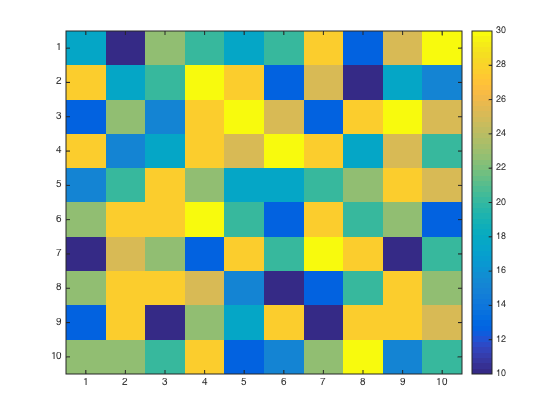
\includegraphics[width=\textwidth]{player_1_best_strategies_V2}
		\caption{Player 1, 100'000 games}
		\label{p1 best strat v2.1}
	\end{subfigure}
	\begin{subfigure}[b]{0.4\textwidth}
		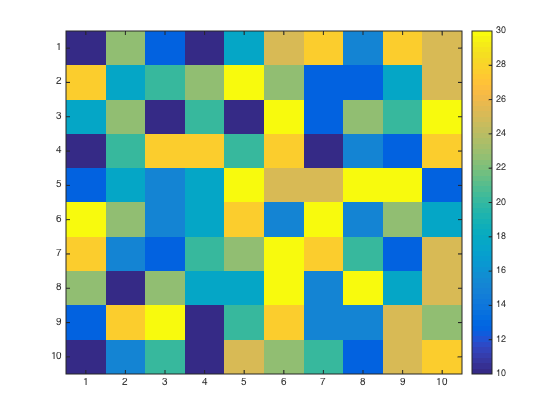
\includegraphics[width=\textwidth]{player_2_best_strategies_V2}
		\caption{Player 2, 100'000 games}
		\label{p2 best strat v2.1}
	\end{subfigure}
	\begin{subfigure}[b]{0.4\textwidth}
		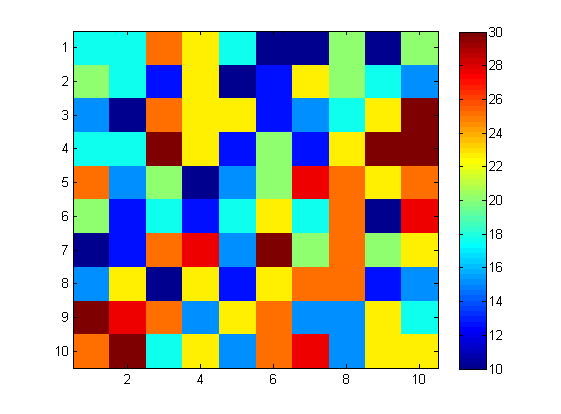
\includegraphics[width=\textwidth]{player_1_best_strategies_V2_2}
		\caption{Player 1, 2'000'000 games}
		\label{p1 best strat v2.2}
	\end{subfigure}
	\begin{subfigure}[b]{0.4\textwidth}
		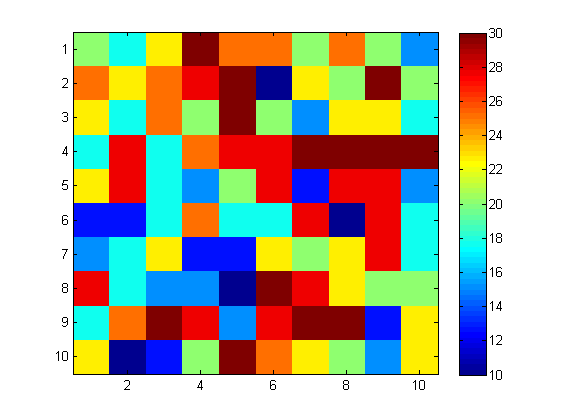
\includegraphics[width=\textwidth]{player_2_best_strategies_V2_2}
		\caption{Player 2, 2'000'000 games}
		\label{p1 best strat v2.2}
	\end{subfigure}
	\caption{Ten best strategies for each player; every row represents a strategy with color-coded percentages.}
	\label{best strat v2}
\end{figure}


\subsection{Version 3: Head \& Tail changes}

\subsubsection{Assumptions \& Implementation}
As our approach with version 2 didn’t lead to a significant result and required too much processing time, we modified the code in a different way. The basic strategy for a player still consists of 10 percentages, each illustrating the amount to invest in every round. But instead of creating a totally random strategy we focus on transformation on the first and last three values, i.e. raising or lowering the ''head'' or ''tail'' of the strategy vector (see Fig. \ref{head tail changes}). This way, a player may invest more or less in the beginning or at the end of a game while the middle stays constant.
\begin{figure}[h]
	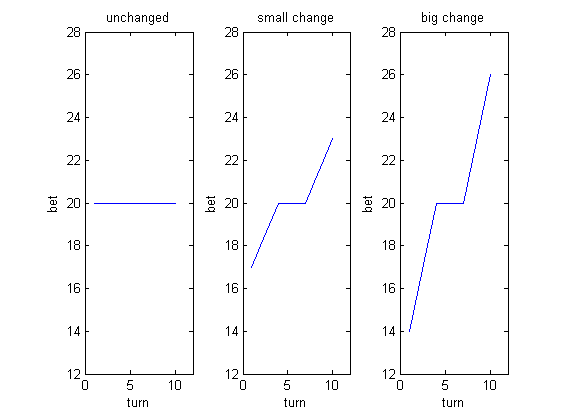
\includegraphics[scale=0.5]{head_tail_changes.png}
	\centering
	\caption{Changes of head and tail}
	\label{head tail changes}
\end{figure}
Both players start with the constant Kelly strategy (betting 20\% in every move). Basically, the two players play a game, each with a defined strategy. Whoever wins sticks to his strategy, whoever loses changes his strategy. If the loser recognize that he lost less badly in the following round he changes his strategy in the same direction as he did before. We quantify the extent of the winning by playing the same round for several times. The player who has won more is the so called winner. The loser has lost less badly when he loses less rounds than before. If he realizes that he lost even worse with the last strategy change, he starts to mutate the tail in one direction. This way, we are trying to quantify how good or bad a strategy is when we modify it in one direction.\\
Whenever a strategy wins we keep it, thus collecting all the potentially good strategies. This makes sure we are always keeping the best strategy which can only be beaten by an even better one. Ideally, a player would keep an optimal strategy forever because nothing can beat it.\\
What's also new compared to the version 2 is that we take into account that players can make mistakes. So we implemented some noise. With a very small probability a player will play a completely different strategy.

\subsubsection{Results \& Discussion}
For a detailed analysis we played the whole game for several times and took the average. The result is shown in Fig. \ref{results v3}. We can not say much out of this data as all the strategies stay very close to Kelly. It seems that strategies with a little higher tail or head may play better than Kelly because their higher riskiness could lead to more money. But the percentages never go far beyond 21\% thus Kelly still seems to be the best strategy.
\begin{figure}
	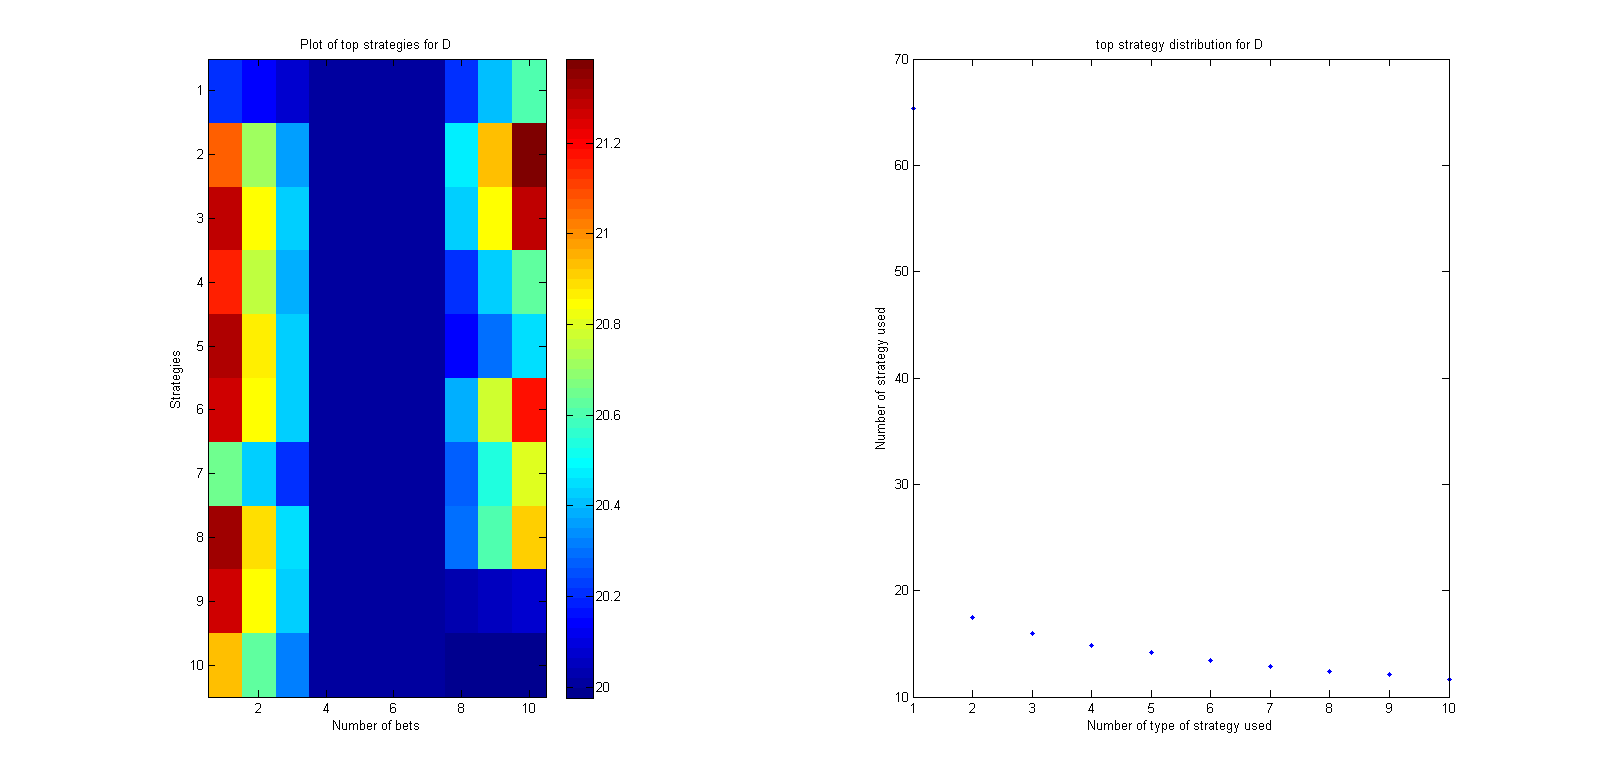
\includegraphics[scale=0.4]{result_V3}
	\centering
	\label{results v3}
	\caption{The ten best strategies for 100 repeats of 1000 rounds of 100 games.}
\end{figure}

\subsection{Version 4: Kelly VS all strategies}
After a last discussion and the results of the previous versions we came back to a very basic game and asked ourselves if there's any strategy that can beat Kelly.

\subsubsection{Assumptions \& Implementation}
One player always plays Kelly, while the other player tries many different strategies to win. We adjust the code so we can plug in the minimum bet, the step size and the maximum bet. After one game (1000 rounds with ten turns per round) player two changes his strategy by adding one step size to the bet of the last turn. \\
We saved and compared the wins of each player. In addition we saved all strategies that won against Kelly.

\subsubsection{Results \& Discussions}
To get good results we should have picked small bet increments of at least 5\% but with an increment so small it would have taken forever to simulate. The number of games can be calculated by $(\frac{top bet-lowest bet}{step size})^{10}$ (for example $((\frac{60\%-30\%}{30\%})+1)^{10}=2^{10}=1024$). So we took large steps of 20\% or even 30\%. The maximum bet we set to 20\% or 30\% and the maximum bet to 60\%. Using these values the simulation was completed within a reasonable time (the run took about one night). To cut down the time we also tried to play less rounds. But with about 100 rounds the results were unusable because they were too random. Reading the graphs (see Fig. \ref{diff v4} \& Fig. \ref{wins v4}) there are some strategies that seem to beat Kelly. The graphs also show that there's a certain trend. Starting with bets much higher or lower than Kelly in the first turns out to be bad for player 2. But if player 2 starts with Kelly and starts to play a little bit more risky towards the end of one round the possibility to win is pretty high.
\begin{figure}[h]
	\centering
	\begin{subfigure}[b]{0.4\textwidth}
		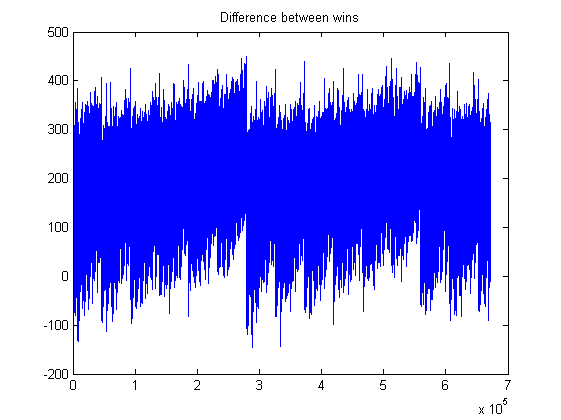
\includegraphics[width=\textwidth]{diff_20_10_70}
		\caption{lowest bet 20\%, step size 10\%, top bet 70\%}
		\label{p1 best strat v2.2}
	\end{subfigure}
	\begin{subfigure}[b]{0.4\textwidth}
		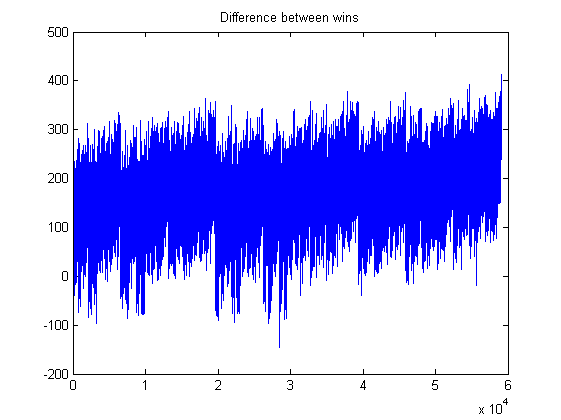
\includegraphics[width=\textwidth]{diff_20_20_60}
		\caption{lowest bet 20\%, step size 20\%, top bet 60\%}
		\label{p1 best strat v2.2}
	\end{subfigure}
	\caption{Differences between the wins of player 1 and 2}
	\label{diff v4}
	
\end{figure}
\begin{figure}[h]
	\centering
	\begin{subfigure}[b]{0.4\textwidth}
		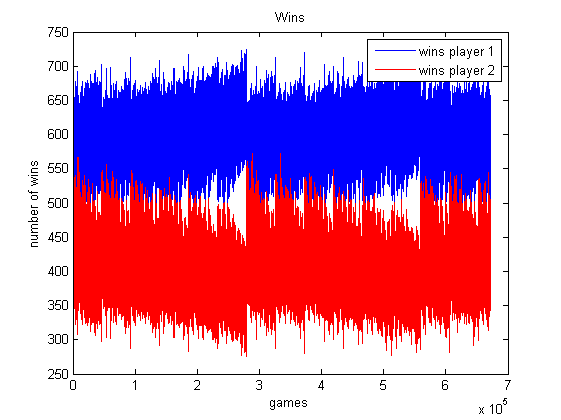
\includegraphics[width=\textwidth]{wins_20_10_70}
		\caption{lowest bet 20\%, step size 10\%, top bet 70\%}
		\label{p1 best strat v2.2}
	\end{subfigure}
	\begin{subfigure}[b]{0.4\textwidth}
		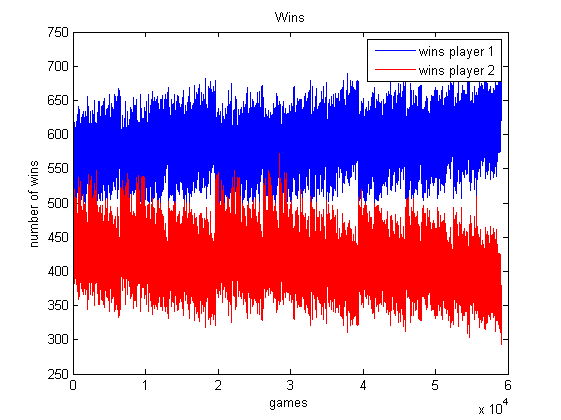
\includegraphics[width=\textwidth]{wins_20_20_60}
		\caption{lowest bet 20\%, step size 20\%, top bet 60\%}
		\label{p1 best strat v2.2}
	\end{subfigure}
	\caption{Wins of player 1 and 2}
	\label{wins v4}
	
\end{figure}
\section{Summary and Outlook}
We all have achieved our goals of this GESS-course: We gained a lot more exercise with Matlab, wrote a structured Latex-report and dived into game theory. Working especially with Matlab was interesting but also very challenging at times. A lot of definitions and decisions had to be made first in order to implement any functional approach. There were many degrees of freedom which were sometimes hard to access and define properly.\\
As for the project problem itself it was always difficult to see whether the data was significant or not. Every approach at least led to results but we can't be sure how much randomness and how much true findings were involved.\\

Version one led us to Kelly which was not surprising as both the players were playing with constant fractions. Then we needed to implement more sophisticated strategies that first had to be defined. This was a crucial point because there is a practically infinite amount of strategies with different parameters. (e.g. dependent on turn \textit{t}, money \textit{m} etc.) Version 2 involved too much randomness and would have taken too long to yield significant data. With version 3 the strategy search got more directed but still seemed to point towards Kelly. Version 4 could have been a good approach but with that little time, implementing, testing and running the code there was no chance to evaluate the results more thoroughly. \\

In retrospect, we think that we have too less know-how in implementing complex models and game theory. So our approaches and models are probably too basic to gain significant data. Especially the learning algorithms (e.g. fictitious play) were too hard for us thus searching efficiently and smart was hardly possible. Furthermore we should have logged more parameters to receive a more significant data evaluation and focus more on interpreting than on simulating. \\

As a further step one should run the codes for a longer period of time. Implementing smarter learning algorithms and more efficient ways to search through the strategy-space would also lead to better results. One could also alter the boundary conditions (e.g. winning probability) as well as extend the problem to N players. \\

As a final step we try to answer our research question. We were trying to find a Nash equilibrium for our problem. Unfortunately we haven't found it because of the reasons which are explained above. We can not say for sure that there is no Nash equilibrium, but with our approaches we did not find it. We can just say that the Kelly strategy (or strategies which are very close to this strategy) still seems to be best one when playing the sequential investment game.

\begin{thebibliography}{9}
	\bibitem{} J. L. Kelly, Jr.: \textit{A New Interpretation of Information Rate}, 1956	
	\bibitem{} Ryan Murphy: \textit{A Sequential Investment Game}, 2011
	\bibitem{} Wikipedia (en): Game Theorie (29.11.2014)
	\bibitem{} Wikipedia (de): Ficticious Play (29.11.2014)
	\bibitem{} Wikipedia (en): Kelly criterion (30.11.2014)
	\bibitem{} Wikipedia (en): John Larry Kelly, Jr. (30.11.2014)
	\bibitem{} Wikipedia (en): Evolutionary Game Theorie (3.12.2014)
	\bibitem{} Discussion with Prof. Dr. Ryan Murphy
\end{thebibliography}

\pagebreak
\appendix
\addcontentsline{toc}{section}{Appendices}
\section*{Appendices}
\section{Matlab code}
\subsection{Version 1}
\subsubsection{SIG\_V1}
\begin{lstlisting}
	% SKRIPTMASTER: Sequential Investment Game for two Players
	%
	% This script contains the code of the Sequential Investment Game for two
	% players, which is part of the GESS course "Modelling and Simulating Social
	% Systems with MATLAB".
	%
	% Authors: Fabian Keller, Sebastian Klotz, Simon Zimmermann
	% Date: 11.11.2014
	% Version 1
	
	clear all
	close all
	clc
	
	% Variable definition
	
	N = 1000;       % number of repeats
	n = 10;         % number of games per repeat
	p = 60;         % winning probability (in %, 0 - 100)
	m_start = 100;  % start amount of money
	
	% Players
	
	bet_1 = zeros(N,1);         % bet player 1 (in %)
	bet_1(1,1) = 5;             % starting bet player 1 (in %)
	bet_2 = zeros(N,1);         % bet player 2 (in %)
	bet_2(1,1) = 25;            % starting bet player 2 (in %)
	score_1 = zeros(N,n+1);     % scores of player 1 in one repeat
	score_2 = zeros(N,n+1);     % scores of player 2 in one repeat
	history_1 = zeros(N,n);     % win (=1) / lose (=0) history of player 
	% 1 in one game (random)
	history_2 = zeros(N,n);     % win (=1) / lose (=0) history of player 
	& 2 in one game (random)    
	win_1 = zeros(N,1);         % win (=1) / lose (=0) history of player 
	% 1 in one repeat   
	win_2 = zeros(N,1);         % win (=1) / lose (=0) history of player 
	% 2 in one repeat
	
	%REF = reference_matrix(10,60);
	
	load('ref.mat');
	
	% Game
	for i = 1:1:N
	score_1(i,1) = m_start;         % first entry = start value
	score_2(i,1) = m_start;         % first entry = start value
	
	for j = 2:1:n+1
	% game for player 1
	rand_Nb_1 = randi(100);
	if rand_Nb_1 <= p           % win
	score_1(i,j) = score_1(i,j-1) + bet_1(i,1)/100*score_1(i,j-1);
	history_1(i,j) = 1;
	else                        % lose
	score_1(i,j) = score_1(i,j-1) - bet_1(i,1)/100*score_1(i,j-1);
	history_1(i,j) = 0;  
	end
	% game for player 2
	rand_Nb_2 = randi(100);
	if rand_Nb_2 <= p           % win
	score_2(i,j) = score_2(i,j-1) + bet_2(i,1)/100*score_2(i,j-1);
	history_2(i,j) = 1;
	else                        % lose
	score_2(i,j) = score_2(i,j-1) - bet_2(i,1)/100*score_2(i,j-1);
	history_2(i,j) = 0;
	end
	end
	
	% Determine win or lose
	
	if score_1(i,11) >= score_2(i,11)
	win_1(i) = 1;
	elseif score_2(i,11) >= score_1(i,11)
	win_2(i) = 1;
	end
	
	% Fictitious Play -> adapt strategy
	if i < N
	[bet_1(i+1,1),bet_2(i+1,1)] = fictitious_play(REF,bet_1(i,1),bet_2(i,1));
	end
	
	end
	
	% Sum of wins
	
	sum_1 = sum(win_1)
	sum_2 = sum(win_2)
	
	if sum_1 > sum_2
	disp('Player 1 wins the game!')
	elseif sum_1 < sum_2
	disp('Player 2 wins the game!')
	else disp('Draw!')
	end
	
	%Plot of scores
	figure(1);
	plot(1:N,score_1(:,11),'b-x')
	hold on
	plot(1:N,score_2(:,11),'r-x')
	xlim([1 N]);
	title('Plot of scores');
	xlabel('Number of game');
	ylabel('Scores');
	legend('Player 1','Player 2');
	
	%Plot of bets
	figure(2);
	plot(1:N,bet_1(:,1),'.b')
	hold on
	plot(1:N,bet_2(:,1),'.r')
	xlim([1 N+1]);
	title('Plot of bets');
	xlabel('Number of game');
	ylabel('bets');
	legend('Player 1','Player 2');
	
	% END OF SIG_V1
\end{lstlisting}
\vspace{10mm}

\subsubsection{Ficticous Play}
\begin{lstlisting}
	% This file contains the "fictitous play"-function for SIG_V1
	
	function[bet_1, bet_2] = fictitious_play(REF, bet_1, bet_2)
	
	% Range
	
	range = 2;
	
	% Player 1:
	
	max_vector_1 = 0;
	max_vector_2 = 0;
	
	max_value_1 = max(REF(2:60, bet_2));
	
	for m = 2:1:60
	if REF(m, bet_2) >= (max_value_1-range)
	if max_vector_1 == 0
	max_vector_1 = m;
	else
	max_vector_1 = [max_vector_1; m];
	end
	end
	end
	
	% Player 2:
	
	max_value_2 = min(REF(bet_1, 2:60));
	
	for m = 2:1:60
	if REF(bet_1, m) <= (max_value_2+range)
	if max_vector_2 == 0
	max_vector_2 = m;
	else
	max_vector_2 = [max_vector_2; m];
	end
	end
	end
	
	bet_1 = max_vector_1( randi( length(max_vector_1) ),1);
	bet_2 = max_vector_2( randi( length(max_vector_2) ) ,1);
	
	if length(max_vector_1) > 1
	max_vector_1;
	elseif length(max_vector_2) > 1
	max_vector_2;
	end
	
	end
	
\end{lstlisting}
\vspace{10mm}

\subsubsection{Reference Matrix}
\begin{lstlisting}
	% This function generates the reference table for both players for SIG_V1
	
	function [REF] = reference_matrix(n, p)
	
	n_table = 10000; % Number of reference plays
	REF = zeros(101,101); % Reference Matrix
	
	for i = 1:1:101
	for j = 1:1:101           
	
	% Game
	for k = 1:1:n_table
	
	money_1 = 100;
	money_2 = 100;
	
	for l = 1:1:n
	% game for player 1
	rand = randi(100);
	if rand <= p           % win
	money_1 = money_1 + (i-1)/100*money_1;
	else                        % lose
	money_1 = money_1 - (i-1)/100*money_1; 
	end
	
	% game for player 2
	rand = randi(100);
	if rand <= p           % win
	money_2 = money_2 + (j-1)/100*money_2;
	else                        % lose
	money_2 = money_2 - (j-1)/100*money_2; 
	end
	end
	
	% write REF
	
	if money_1 > money_2
	REF(i,j) = REF(i,j) + 1;
	elseif money_2 > money_1
	REF(i,j) = REF(i,j) - 1;                
	end
	
	end
	
	end
	end
	
	figure
	imagesc(REF)
	
	end
\end{lstlisting}
\pagebreak

\subsection{Version 2}
\begin{lstlisting}
	% SKRIPTMASTER: Sequential Investment Game for two Players
	%
	% This script contains the code of the Sequential Investment Game for two
	% players, which is part of the GESS course "Modelling and Simulating Social
	% Systems with MATLAB".
	%
	% Authors: Fabian Keller, Sebastian Klotz, Simon Zimmermann
	% Date: 25.11.2014
	% Version 2
	
	clear all
	close all
	clc
	
	% Variable definition
	
	c = 100;                    % number of repeats
	C = 100;                    % number of games
	n = 10;                     % number of turns
	
	m_start = 100;              % starting money
	p = 60;                     % probability of winning in %
	
	s_pool = 10:2.5:30;         % pool of bets
	
	strategy_1 = zeros(1,n);    % strategies: 10x bet
	strategy_2 = zeros(1,n);
	win_1 = zeros(1,2);         % wins | uses - per strategy
	win_2 = zeros(1,2);
	money_1 = zeros(1);         % money
	money_2 = zeros(1);
	
	% start strategy
	for l = 1:1:n
	strategy_1(1,l) = s_pool(randi(length(s_pool)));
	end
	for l = 1:1:n
	strategy_2(1,l) = s_pool(randi(length(s_pool)));
	end
	
	% SIG
	for i = 1:1:C
	
	% round
	for j = 1:1:c
	
	money_1(end) = m_start;
	money_2(end) = m_start;
	
	% turn
	for k = 1:1:n
	
	% player 1
	if randi(100) <= p
	money_1(end) = money_1(end) + money_1(end)*strategy_1(end,k)/100;
	else
	money_1(end) = money_1(end) - money_1(end)*strategy_1(end,k)/100;
	end
	
	% player 2
	if randi(100) <= p
	money_2(end) = money_2(end) + money_2(end)*strategy_2(end,k)/100;
	else
	money_2(end) = money_2(end) - money_2(end)*strategy_2(end,k)/100;
	end
	
	end
	
	% Who has won?
	if money_1(end) > money_2(end)
	win_1(end,1) = win_1(end,1) + 1;
	elseif money_1(end) < money_2(end)
	win_2(end,1) = win_2(end,1) + 1;
	end
	
	end
	
	% strategy change
	if win_1(end,1) > win_2(end,1)
	% player 2 change
	win_2(end+1,1) = 0;
	money_2(end+1) = 0;
	strategy_2(end+1,:) = 0;
	for l = 1:1:n
	strategy_2(end,l) = s_pool(randi(length(s_pool)));
	end
	elseif win_1(end,1) < win_2(end,1)
	% player 1 change
	win_1(end+1,1) = 0;
	money_1(end+1) = 0;
	strategy_1(end+1,:) = 0;
	for l = 1:1:n
	strategy_1(end,l) = s_pool(randi(length(s_pool)));
	end
	end
	
	% counter reset
	win_1(end,1) = 0;
	win_2(end,1) = 0;
	
	% number of rounds a strategy has been used
	win_1(end,2) = win_1(end,2) + 1;
	win_2(end,2) = win_2(end,2) + 1;
	
	end
	
	disp('Finished.')
	disp(' ')
	disp('Number of loops done:')
	i*j*k
	
	disp(' ')
	disp('Analysis of strategies:')
	disp(' ')
	
	% strategy used the most:
	[max_val_1,max_ind_1] = max(win_1(:,2));
	[max_val_2,max_ind_2] = max(win_2(:,2));
	disp('Strategies used the most:')
	disp(' ')
	disp('Player 1')
	Strategy = strategy_1(max_ind_1,:)
	used = max_val_1
	disp('Player 2')
	Strategy = strategy_2(max_ind_2,:)
	used = max_val_2
	disp(' ')
	disp('end')
	
	% order arrays and imagesc strategies
	[sort_val_1,sort_ind_1] = sort(win_1(:,2), 'descend');
	[sort_val_2,sort_ind_2] = sort(win_2(:,2), 'descend');
	
	% Plot of strategies
	figure(1)
	subplot(1,2,1)
	imagesc(strategy_1(sort_ind_1(1:10),:))
	title('Plot of top strategies of player 1');
	xlabel('Number of bets');
	ylabel('Strategies');
	colorbar
	subplot(1,2,2)
	imagesc(strategy_2(sort_ind_2(1:10),:))
	title('Plot of top strategies of player 2');
	xlabel('Number of bets');
	ylabel('Strategies');
	colorbar
	
	% END OF SIG_V2
\end{lstlisting}
\vspace{10mm}

\subsection{Version 3}
\begin{lstlisting}
	% SKRIPTMASTER: Sequential Investment Game for two Players
	%
	% This script contains the code of the Sequential Investment Game for two
	% players, which is part of the GESS course "Modelling and Simulating Social
	% Systems with MATLAB".
	%
	% Authors: Fabian Keller, Sebastian Klotz, Simon Zimmermann
	% Date: 08.12.2014
	% Version 3
	
	clear all
	clc
	close all
	
	% Variable definition
	
	D = 100;                    % repeats of one game
	%N = 100;                   % number of repeats
	N = 1000;
	g = 100;                    % number of games per repeat
	n = 10;                     % number of rounds per game
	
	m_start = 100;              % starting money
	p = 60;                     % probability of winning in %
	c = 0;                      % number of games since last strategy change
	c_max = 0;                  % max round of strategy kept
	winner = 0;                 % winner of last game (1 or 2)
	median = 0;                 % median
	strategy = 0;               % which strategy the loser chooses (row of matrix)
	row = 1;                    % row of strategy_matrix
	noise = N/40;               % noise factor
	noise_1 = 0;                % noise factor of player 1
	noise_2 = 0;                % noise factor of player 2
	
	s_min = 2;
	s_max = 80;
	
	win_1 = 0;                  % player 1 wins total
	win_2 = 0;                  % player 2 wins total
	row_1 = 0;                  % Strategy-N? P1
	row_2 = 0;
	
	% Matrix of mutations
	strategy_matrix = [3 2 1 0 0 0 0 0 0 0;
	-3 -2 -1 0 0 0 0 0 0 0;
	0 0 0 0 0 0 0 1 2 3;
	0 0 0 0 0 0 0 -1 -2 -3];
	
	strategy_matrix = strategy_matrix/5;
	
	strategy_kelly = [20 20 20 20 20 20 20 20 20 20];
	
	strategy_matrix_1 = zeros(N,n);
	strategy_matrix_2 = zeros(N,n);
	
	strategy_1 = strategy_kelly;
	strategy_2 = strategy_kelly;
	
	strategy_matrix_w = zeros(N,n);
	
	% VARIABLES DATASET
	
	top_10_number = zeros(10,1);
	top_10_win_strategies = zeros(10,10);
	top_10 = zeros(10,1);
	
	% ----------
	%    GAME   
	% ----------
	
	for d = 1:1:D
	
	% starting strategies
	
	strategy_1 = strategy_kelly;
	strategy_2 = strategy_kelly;
	
	i = 1;
	
	while(i <= N)
	% repeat
	
	w_1 = 0;  % wins player 1 per repeat (NOT total)
	w_2 = 0;
	
	% Noise
	noise = noise - 1;
	
	% For player 1
	if randi(N) <= noise
	strategy_1 = strategy_kelly;
	
	noise_1 = noise_1 + 1;
	
	for j = 1:1:size(strategy_matrix,1)
	strategy_1 = strategy_1 + randi(3)*strategy_matrix(j,:);
	end
	
	end
	
	% For player 2
	
	if randi(N) <= noise
	strategy_2 = strategy_kelly;
	
	noise_2 = noise_2 + 1;
	
	for j = 1:1:size(strategy_matrix,1)
	strategy_2 = strategy_2 + randi(3)*strategy_matrix(j,:);
	end
	
	end
	
	for j = 1:1:g
	%game
	
	m_1 = m_start;
	m_2 = m_start;
	
	for k = 1:1:n
	% round
	
	% player 1
	if randi(100) <= p
	m_1 = m_1 + m_1*strategy_1(k)/100;
	else
	m_1 = m_1 - m_1*strategy_1(k)/100;
	end
	
	% player 2
	if randi(100) <= p
	m_2 = m_2 + m_2*strategy_2(k)/100;
	else
	m_2 = m_2 - m_2*strategy_2(k)/100;
	end
	
	end
	
	% wins
	
	if m_1 > m_2
	w_1 = w_1 + 1;
	elseif m_2 > m_1
	w_2 = w_2 + 1;
	end
	
	end
	
	% strategy change
	
	if w_1 > w_2 
	% PLAYER 1 WINS
	
	% player 1 sticks to strategy
	win_1 = win_1 + 1;
	strategy_matrix_w(i,:) = strategy_1;
	
	if winner == 1
	% AGAIN
	
	c = c + 1; 
	median_old = median;
	median = (median_old*(c-1) + w_1 - w_2)/c;
	
	else
	% FIRST TIME
	
	if c > c_max
	c_max = c;
	end
	
	c = 1;
	winner = 1;
	median_old = g;
	median = w_1 - w_2;
	
	end
	
	% Player 2 mutatates
	
	if median_old <= median
	% improved strategy -> continue
	
	if strategy_2(1) >= s_min && strategy_2(n) >= s_min 
	&& strategy_2(1) <= s_max && strategy_2(n) <= s_max
	strategy_2 = strategy_2 + strategy;
	end
	
	else
	% new strategy
	
	if c > 1 && strategy_2(1) >= s_min && strategy_2(n) >= s_min
	 && strategy_2(1) <= s_max && strategy_2(n) <= s_max
	% revert changes 
	strategy_2 = strategy_2 - strategy;
	end
	
	if row_2 <= 2
	row_2 = randi([3,4]); % tail
	else
	row_2 = randi([1,2]); % head
	end
	
	strategy = strategy_matrix(row_2,:);
	
	if strategy_2(1) >= s_min && strategy_2(n) >= s_min 
	&& strategy_2(1) <= s_max && strategy_2(n) <= s_max
	strategy_2 = strategy_2 + strategy;
	end
	
	end
	
	elseif w_2 > w_1
	% PLAYER 2 WINS
	
	% player 2 sticks to strategy
	win_2 = win_2 + 1;
	strategy_matrix_w(i,:) = strategy_1;
	
	if winner == 2
	% AGAIN
	
	c = c + 1; 
	median_old = median;
	median = (median_old*(c-1) + w_2 - w_1)/c;
	
	else
	% FIRST TIME
	
	if c > c_max
	c_max = c;
	end
	
	c = 1;
	winner = 2;
	median_old = g;
	median = w_2 - w_1;
	
	end
	
	% Player 1 mutatates
	
	if median_old <= median
	% improved strategy -> continue
	
	if strategy_1(1) >= s_min && strategy_1(n) >= s_min
	 && strategy_1(1) <= s_max && strategy_1(n) <= s_max
	strategy_1 = strategy_1 + strategy;
	end
	
	else
	% new strategy
	
	if c > 1 && strategy_1(1) >= s_min && strategy_1(n) >= s_min 
	&& strategy_1(1) <= s_max && strategy_1(n) <= s_max
	% revert changes 
	strategy_1 = strategy_1 - strategy;
	end
	
	if row_1 <= 2
	row_1 = randi([3,4]); % tail
	else
	row_1 = randi([1,2]); % head
	end
	
	strategy = strategy_matrix(row_1,:);
	
	if strategy_1(1) >= s_min && strategy_1(n) >= s_min 
	&& strategy_1(1) <= s_max && strategy_1(n) <= s_max
	strategy_1 = strategy_1 + strategy;
	end
	
	end
	
	end
	
	strategy_matrix_1(i,:) = strategy_1;    % log
	strategy_matrix_2(i,:) = strategy_2;    % log
	
	if w_1 == w_2
	% draw
	
	% "mark" row
	strategy_matrix_w(i,:) = 0;
	
	% repeat loop
	i = i-1;
	end
	
	i = i + 1; % index variable
	
	end
	
	B = sortrows(strategy_matrix_w);
	S = [1;any(diff(B),2)];
	[L,S] = regexp(sprintf('%i',S'),'1(0)+');
	repeated_rows = B(S,:);             % Repeated Rows.
	repeat_count = (S-L+1)';            % How often each repeated row appears.
	
	[sort_val_1,sort_ind_1] = sort(repeat_count, 'descend');
	
	length(sort_val_1)
	
	if length(sort_val_1) >= 10
	top_10 = sort_val_1(1:10);
	top_10_number = top_10_number + top_10;
	
	top_10_strategies = repeated_rows(sort_ind_1(1:10),:);
	top_10_win_strategies = top_10_win_strategies + top_10_strategies;
	end
	
	end
	
	top_10_number = top_10_number / D
	top_10_win_strategies = top_10_win_strategies/D
	
	% Plots
	figure(1)
	subplot(1,2,1)
	imagesc(top_10_win_strategies)
	title('Plot of top strategies for D');
	xlabel('Number of bets');
	ylabel('Strategies');
	colorbar
	subplot(1,2,2)
	plot(top_10_number, '.')
	title('top strategy distribution for D');
	xlabel('Number of type of strategy used');
	ylabel('Number of strategy used');
\end{lstlisting}
\vspace{10mm}

\subsection{Version 4}
\begin{lstlisting}
	% SKRIPTMASTER: Sequential Investment Game for two Players
	%
	% This script contains the code of the Sequential Investment Game for two
	% players, which is part of the GESS course "Modelling and Simulating Social
	% Systems with MATLAB".
	%
	% Authors: Fabian Keller, Sebastian Klotz, Simon Zimmermann
	% Date: 08.12.2014
	% Version 4
	
	close all
	clear all
	clc
	
	%--------------------------------------%
	% variables
	%--------------------------------------%
	
	g=0;                    %number of games
	r=1000;                 %number of rounds per gae
	t=10;                   %number of turns per romund
	p=60;                   %probability to win [%]
	k=100;                  %amount of currency each player starts with
	lowest_bet=20;          %in [%]
	step_size=2;            %in [%]
	top_bet=26;             %in [%]
	log_nr=0;               %log counter
	strategy_matrix_w = zeros(1,12); % log of winning strategies
	c = 0;                  % counter for strategy_matrix_w
	
	%win=zeros(r,2);        %matrix with wins
	win1=0;
	win2=0;
	strat=zeros(1,10);      %bets of player 2 for every turn (each turn = column)
	%start_value=20;        %value for the bets of player two to start from
	
	%--------------------------------------%
	%fill strat with start values
	%--------------------------------------%
	
	for i=1:1:10
	strat(1,i)=lowest_bet;
	end
	
	%--------------------------------------%
	%play the game
	%--------------------------------------%
	f=0;
	
	while f==0
	g=g+1
	strat_log=zeros(g,11); %log of the strategy matrix that won against 
	% kelly and in which game
	
	%generate all possbile strategies
	if (strat(1,1)==top_bet)&&(strat(1,2)==top_bet)&&(strat(1,3)==top_bet)
	&&(strat(1,4)==top_bet)&&(strat(1,5)==top_bet)&&(strat(1,6)==top_bet)
	&&(strat(1,7)==top_bet)&&(strat(1,8)==top_bet)&&(strat(1,9)==top_bet)
	&&(strat(1,10)==top_bet)
	f=1;
	else
	if (strat(1,2)==top_bet)&&(strat(1,3)==top_bet)&&(strat(1,4)==top_bet)
	&&(strat(1,5)==top_bet)&&(strat(1,6)==top_bet)&&(strat(1,7)==top_bet)
	&&(strat(1,8)==top_bet)&&(strat(1,9)==top_bet)&&(strat(1,10)==top_bet)
	strat(1,1)=strat(1,1)+step_size;
	strat(1,2)=lowest_bet;
	strat(1,3)=lowest_bet;
	strat(1,4)=lowest_bet;
	strat(1,5)=lowest_bet;
	strat(1,6)=lowest_bet;
	strat(1,7)=lowest_bet;
	strat(1,8)=lowest_bet;
	strat(1,9)=lowest_bet;
	strat(1,10)=lowest_bet;
	else
	if (strat(1,3)==top_bet)&&(strat(1,4)==top_bet)&&(strat(1,5)==top_bet)
	&&(strat(1,6)==top_bet)&&(strat(1,7)==top_bet)&&(strat(1,8)==top_bet)
	&&(strat(1,9)==top_bet)&&(strat(1,10)==top_bet)
	strat(1,2)=strat(1,2)+step_size;
	strat(1,3)=lowest_bet;
	strat(1,4)=lowest_bet;
	strat(1,5)=lowest_bet;
	strat(1,6)=lowest_bet;
	strat(1,7)=lowest_bet;
	strat(1,8)=lowest_bet;
	strat(1,9)=lowest_bet;
	strat(1,10)=lowest_bet;
	else
	if (strat(1,4)==top_bet)&&(strat(1,5)==top_bet)&&(strat(1,6)==top_bet)
	&&(strat(1,7)==top_bet)&&(strat(1,8)==top_bet)&&(strat(1,9)==top_bet)
	&&(strat(1,10)==top_bet)
	strat(1,3)=strat(1,3)+step_size;
	strat(1,4)=lowest_bet;
	strat(1,5)=lowest_bet;
	strat(1,6)=lowest_bet;
	strat(1,7)=lowest_bet;
	strat(1,8)=lowest_bet;
	strat(1,9)=lowest_bet;
	strat(1,10)=lowest_bet;
	else
	if (strat(1,5)==top_bet)&&(strat(1,6)==top_bet)&&(strat(1,7)==top_bet)
	&&(strat(1,8)==top_bet)&&(strat(1,9)==top_bet)&&(strat(1,10)==top_bet)
	strat(1,4)=strat(1,4)+step_size;
	strat(1,5)=lowest_bet;
	strat(1,6)=lowest_bet;
	strat(1,7)=lowest_bet;
	strat(1,8)=lowest_bet;
	strat(1,9)=lowest_bet;
	strat(1,10)=lowest_bet;
	else
	if (strat(1,6)==top_bet)&&(strat(1,7)==top_bet)&&(strat(1,8)==top_bet)
	&&(strat(1,9)==top_bet)&&(strat(1,10)==top_bet)
	strat(1,5)=strat(1,5)+step_size;
	strat(1,6)=lowest_bet;
	strat(1,7)=lowest_bet;
	strat(1,8)=lowest_bet;
	strat(1,9)=lowest_bet;
	strat(1,10)=lowest_bet;
	else
	if (strat(1,7)==top_bet)&&(strat(1,8)==top_bet)&&(strat(1,9)==top_bet)
	&&(strat(1,10)==top_bet)
	strat(1,6)=strat(1,6)+step_size;
	strat(1,7)=lowest_bet;
	strat(1,8)=lowest_bet;
	strat(1,9)=lowest_bet;
	strat(1,10)=lowest_bet;
	else
	if (strat(1,8)==top_bet)&&(strat(1,9)==top_bet)&&(strat(1,10)==top_bet)
	strat(1,7)=strat(1,7)+step_size;
	strat(1,8)=lowest_bet;
	strat(1,9)=lowest_bet;
	strat(1,10)=lowest_bet;
	else
	
	if (strat(1,9)==top_bet)&&(strat(1,10)==top_bet)
	strat(1,8)=strat(1,8)+step_size;
	strat(1,9)=lowest_bet;
	strat(1,10)=lowest_bet;
	
	else
	if strat(1,10)==top_bet
	strat(1,9)=strat(1,9)+step_size;
	strat(1,10)=lowest_bet;
	else
	strat(1,10)=strat(1,10)+step_size;
	end
	end
	end
	end
	end
	end
	end
	end
	end
	end
	
	for i=1:1:r
	k1=k;
	k2=k;
	for j=1:1:t
	
	%player 1
	rand1=randi(100,1,1);
	if rand1 <= p
	k1=k1+(0.2*k1);
	else
	k1=k1-(0.2*k1);
	end
	
	%player 2
	rand2=randi(100,1,1);
	if rand2 <= p
	k2=k2+((strat(1,j)*k2)/100);
	else
	k2=k2-((strat(1,j)*k2)/100);
	end
	
	
	
	end
	
	if k1 > k2           %player 1 wins the round
	%             win(i,1)=1;
	%             win(i,2)=0;
	win1=win1+1;
	else                 %player 2 wins the round
	%             win(i,2)=1;
	%             win(i,1)=0;
	win2=win2+1;
	end
	
	end   
	
	%     win1=sum(win(:,1));
	%     win2=sum(win(:,2));
	
	
	diff(1,g)=win1-win2;
	
	%     if win2 <= win1
	%         log_nr=log_nr+1;
	%         strat_log(log_nr,11)=g;
	
	win(1,g)=win1;
	win(2,g)=win2;
	
	if win2 > win1
	c = c + 1;
	for j = 1:1:10
	strategy_matrix_w(c,j) = strat(1,j);
	strategy_matrix_w(c,11) = win2;
	strategy_matrix_w(c,12) = g;
	end
	end
	
	win1=0;
	win2=0;
	
	clc
	
	end
	
	figure(1)
	plot(diff)
	title('Difference between wins')
	
	figure(2)
	plot(win(1,:),'b')
	hold on
	plot(win(2,:),'r')
	legend('wins player 1','wins player 2')
	title('Wins')
	xlabel('games')
	ylabel('number of wins')
	
	% END OF SIG_V4
\end{lstlisting}


\end{document} 
